\documentclass[../main.tex]{subfiles}
\chapter{Validierung}
\label{c:validierung}

Die Beschreibung der Kinematik der Maschine erfolgt mit einer homogenen Transformationsmatrix je Freiheitsgrad.
Die der Simulation zugrunde liegende Maschine hat 6 geführte Freiheitsgrade.
Von diesen sind 4 über einen Vorschub an die Drehzahl des Werkzeugs gekoppelt.
Die positive Richtung dieser Freiheitsgrade ist außerdem nicht streng anhand der mathematisch positive Richtung des Standardkoordinatensystems definiert.
Um Vorzeichen-, Drehmittelpunkts- und Fehler in der Anwendungsreihenfolge der Abbildungsmatrizen zu verhindern ist eine visuelle Validierung der in Kap.\ \ref{c:herleitung} entwickelten linearen Algebra anhand einer erprobten Methode also sinnvoll.
Diese Methode sollte Teil der \matlab Toolchain sein, erlauben das Modell extern zu bedaten und eine grafische Ausgabe zur Verfügung stellen.
Es wurde entschieden das kinematische Modell als Simscape Multibody Modell aufzubauen.
Bei Simscape\texttrademark\xspace handelt es sich um eine Reihe von Blockbibliotheken und speziellen Simulationsfunktionen zur Modellierung physikalischer Systeme in der Simulink\textregistered-Umgebung.
Sie verwendet den Physical Network-Ansatz, der sich von dem Standard-Simulink-Modellierungsansatz unterscheidet und sich besonders für die Simulation von Systemen eignet, die aus realen physikalischen Komponenten bestehen. \cite{mwSim}
Vergleichbar zu Simulink wird hier ein Signalflussplan erstellt, der die Wechselwirkung von, zu Blöcken zusammengefassten, Funktionsgruppen mit Hilfe von Verbindungen beschriebt.
Diese Verbindungen stellen in Simulink Signale dar, üblicherweise zeitdiskrete Zahlenwerte oder logische Zustände.
In Simscape stellen diese Verbindungen allerdings die Position und Ausrichtung eines Koordinatensystems im world-Koordinatensystem, dem Ursprung des Modells, dar.
Diese verschiedenen Formen der Modellierung können in einem Blockschaltbild koexistieren und mit Hilfe von "Physical Signal Converters" vereint werden.
So kann ein Simulink-Signal in eine zeitdiskrete Transformation eines Koordinatensystem gewandelt werden, oder Position und Ausrichtung eines Koordinatensystems in einem Signal erfasst werden.

\section{Mechanisches Modell der Maschine}

Anhand der schematischen Darstellung einer Wälzfräsmaschine in Abb.\ \ref{fig:maschine} wurde in Creo Parametric eine dreidimensionales Modell erstellt.
Die Komponenten der Maschine wurden im Mechanismus-Modus zu einem kinematischen Modell verknüpft.
Dieses kinematische CAD-Modell wurde anschließend mittels einer Softwareschnittstelle in ein Simscape Multibody Modell konvertiert.

Ursprung des CAD-Modells ist das Maschinenbett-Koordinatensystem.
Anfänglich wurden alle Komponenten der Maschine auf dieses Standard-Koordinatensystem konstruiert.
Nach Konvertierung der CAD-Komponenten in ein neutrales Datenformat beinhalten alle Teile dieses Koordinatensystem als Ursprung.
Dadurch sollte der Aufbau des Simscale Modells vereinfachen werden, da alle Komponenten ohne linearen oder rotatorischen Versatz auf des world-Koordinatensystem referenziert werden können.

\begin{figure}
	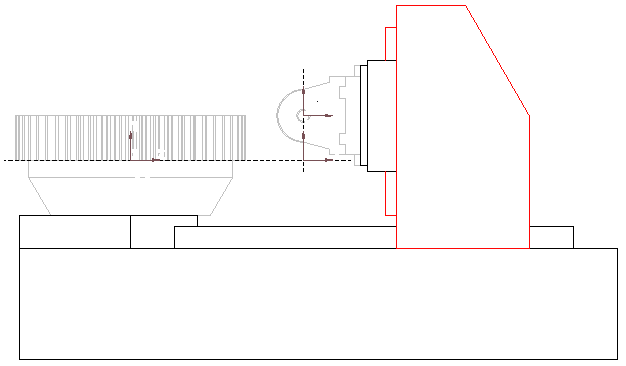
\includegraphics{skelettmodell}
	\caption{Konstruktion des Koordinatensystems für Schlitten in x-Richtung}
	\label{fig:skelettmodell}
\end{figure}

Die in Simscape zur Verfügung stehenden Blöcke verwenden als primäre Achse allerdings immer die z-Achse; Translationen können ausschließlich entlang der z-Achse erfolgen, Rotationen ausschließlich um diese herum.
Es ist also notwendig den Komponenten zweckmäßige und individuelle Koordinatensysteme aufzuprägen.
Als Ursprung für ein solches Koordinatensystem bietet sich der Schnittpunkt von Hauptachsen der Koordinatensystem der Mutter- und Tochter-Komponenten (vgl. Abb.\ \ref{fig:skelettmodell}).
Die Ausrichtung sollte mit Blick auf die Transformation der Tochter-Komponenten so gewählt werden, dass keine weitere Transformation innerhalb der Komponente notwendig ist.
In Abbildung \ref{fig:skelettmodell} ist die Konstruktion des Koordinatensystems für den Maschinenschlitten der x-Achse (mit roter Umrandung) dargestellt.
Das in der kinematischen Kette vor dieser Komponente liegende Bauteil, das Maschinenbett, übergibt ein Koordinatensystem mit z-Achse in Richtung des x-Achsen-Freiheitsgrades.
Das Koordinatensystem muss also um einen Offset verschoben und so gedreht werden, dass die z-Achse auf der Ausgangsseite in Richtung des Maschinen-Z-Freiheitsgrades zeigt.
Das Koordinatensystem des in der kinematischen Kette nachfolgend liegende Teiles, der Schlitten der z-Achse ist dann wiederum translatorisch verschoben, damit der Ursprung auf der Rotationsachse der Werkzeugspindel liegt.
Dieses muss dann im nächsten Schritt noch so gedreht werden, dass die z-Achse in Richtung der Rotationsachse der A-Achse zeigt.

Eine mechanische Komponente wird innerhalb von Simscape als "File Solid block" repräsentiert.
Dieser Block hat, wie andere mechanische Blöcke, einen Koordinatensystem-Eingang und es können ein oder mehrere Ausgänge ergänzt werden.
Maskiert innerhalb des Blockes kann eine feste Transformation von Eingang zu Ausgangskoordinatensystem definiert werden.
